\documentclass[12pt]{article}
\usepackage[utf8]{inputenc}
\usepackage{graphicx}
\usepackage{multicol}
\usepackage{listings}
\usepackage{amsmath}
\graphicspath{ {./images/} }
\usepackage{amssymb}
\usepackage[htt]{hyphenat}

\usepackage{hyperref}
\hypersetup{
    colorlinks=true,
    linkcolor=blue,
    filecolor=magenta,      
    urlcolor=cyan,
}

\usepackage{xcolor}

\definecolor{codegreen}{rgb}{0,0.6,0}
\definecolor{codegray}{rgb}{0.5,0.5,0.5}
\definecolor{codepurple}{rgb}{0.58,0,0.82}
\definecolor{backcolour}{rgb}{0.95,0.95,0.92}
\definecolor{codeorange}{rgb}{1,0.64,0}

\lstdefinestyle{mystyle}{
    backgroundcolor=\color{backcolour},   
    commentstyle=\color{codegreen},
    keywordstyle=\color{magenta},
    numberstyle=\tiny\color{codeorange},
    stringstyle=\color{codepurple},
    basicstyle=\ttfamily\footnotesize,
    breakatwhitespace=false,         
    breaklines=true,                 
    captionpos=b,                    
    keepspaces=true,                 
    numbers=left,                    
    numbersep=5pt,                  
    showspaces=false,                
    showstringspaces=false,
    showtabs=false,                  
    tabsize=2
}

\lstset{style=mystyle, breaklines=true, postbreak=\mbox{\textcolor{red}{$\hookrightarrow$}\space}}

\title{\vspace{-1cm}The Laplace Transform\\
\large Assignment 6\\
\large EE2703 - Applied Programming Lab}
\author{Abhigyan Chattopadhyay \\
EE19B146}
\date{18th April 2021}
\usepackage[margin=0.75in]{geometry}

\begin{document}
\maketitle
\tableofcontents
\pagebreak
\section{The Problem at Hand}
We want to analyse the frequency responses of various given input signals using the \texttt{scipy.signal} module in python.

\subsection{The Laplace Transform}
The Laplace Transform of a function takes the function in the time domain and converts it to its frequency domain representation in the Complex plane.

The equation for the (bilateral) Laplace Transform of a function $f(x)$ is:

$$F(s) = \int_{-\infty}^{\infty} f(t) e^{-st} dt$$

It also has some properties, of which we will be using the Derivative Property later on.

\section{Solutions to given Questions}

\subsection{Question 1: Impulse Response of a Damped Spring System}

We are given that a spring satisfying the equation:

$$\ddot x + 2.25x = f(t)$$

And it is acted upon by the forcing function:
$$f(t) = \cos(1.5t)e^{-0.5t}u_0(t)$$

The Laplace Transform of the given forcing function is given by:
$$F(s) = \frac{s+0.5}{(s+0.5^2)+2.25}$$

We will try to solve this over the time interval from 0 to 50 seconds using the \texttt{system.impulse} function as follows:

\begin{lstlisting}[language=Python]
def main():
    F1 = transfer(0.5,1.5)
    X1 = LTIMore([1,0,2.25],[1])
    H1 = F1/X1
    times = np.linspace(0,50,1000)
    ts,xs = sp.impulse(H1,None,times)
    oneshotplot(1,ts,xs,title="Plot for Question 1")
\end{lstlisting}

Note that some custom functions and classes were used here, which are defined in the \texttt{Assignment\_6.py} file. They are also given here for reference and they are explained in the comments:

\begin{lstlisting}[language=Python]
import numpy as np
import scipy.signal as sp
import matplotlib.pyplot as plt
from scipy.signal.ltisys import TransferFunctionContinuous as TransFun
class LTIMore(TransFun):
    def __neg__(self):
        return LTIMore(-self.num,self.den)
    def __mul__(self,other):
        if type(other) in [int,float]:
            return LTIMore(self.num*other,self.den)
        elif type(other) in [TransFun,LTIMore]:
            n = np.polymul(other.num,self.num)
            d = np.polymul(other.den,self.den)
            return LTIMore(n,d)
    
    def __truediv__(self,other):
        if type(other) in [int,float]:
            return LTIMore(self.num,self.den*other)
        elif type(other) in [TransFun,LTIMore]:
            n = np.polymul(other.den,self.num)
            d = np.polymul(other.num,self.den)
            return LTIMore(n,d)
    
    def __rtruediv__(self,other):
        if type(other) in [int,float]:
            return LTIMore(self.den*other,self.num)
        elif type(other) in [TransFun,LTIMore]:
            n = np.polymul(self.den,other.num)
            d = np.polymul(self.num,other.den)
            return LTIMore(n,d)
    
    def __add__(self,other):
        if type(other) in [int,float]:
            return LTIMore(np.polyadd(self.num,other*self.den),self.den)
        elif type(other) in [TransFun,LTIMore]:
            n = np.polyadd(np.polymul(self.den,other.num),np.polymul(self.num,other.den))
            d = np.polymul(self.den,other.den)
            return LTIMore(n,d)
    
    def __sub__(self,other):
        return self + (-other)
    def __rsub__(self,other):
        return (-self) + other

def transfer(alpha,omega):
    return LTIMore([1,alpha],[1,2*alpha,omega**2+alpha**2])

def oneshotplot(i,x,y,xlabel='t',ylabel='x',title="Fig"):
    """To Plot Graphs in one single function"""
    plt.figure(i)
    plt.plot(x,y,"-r")
    plt.xlabel(xlabel)
    plt.ylabel(ylabel)
    plt.title(title)
    plt.savefig("fig"+str(i),dpi=1000)
    plt.show()
\end{lstlisting}


In essence, the LTIMore class adds the functionality of addition, subtraction, multiplication and division to the vanilla \texttt{scipy.signal.lti.TransferFunctionContinuous} class and allows for easy manipulation of the transfer functions.

The \texttt{oneshotplot} function allows us to plot a graph with a specified title and labels all in one line instead of calling each individual \texttt{pyplot} command.

\pagebreak
We obtain the following graph:

\begin{center}
    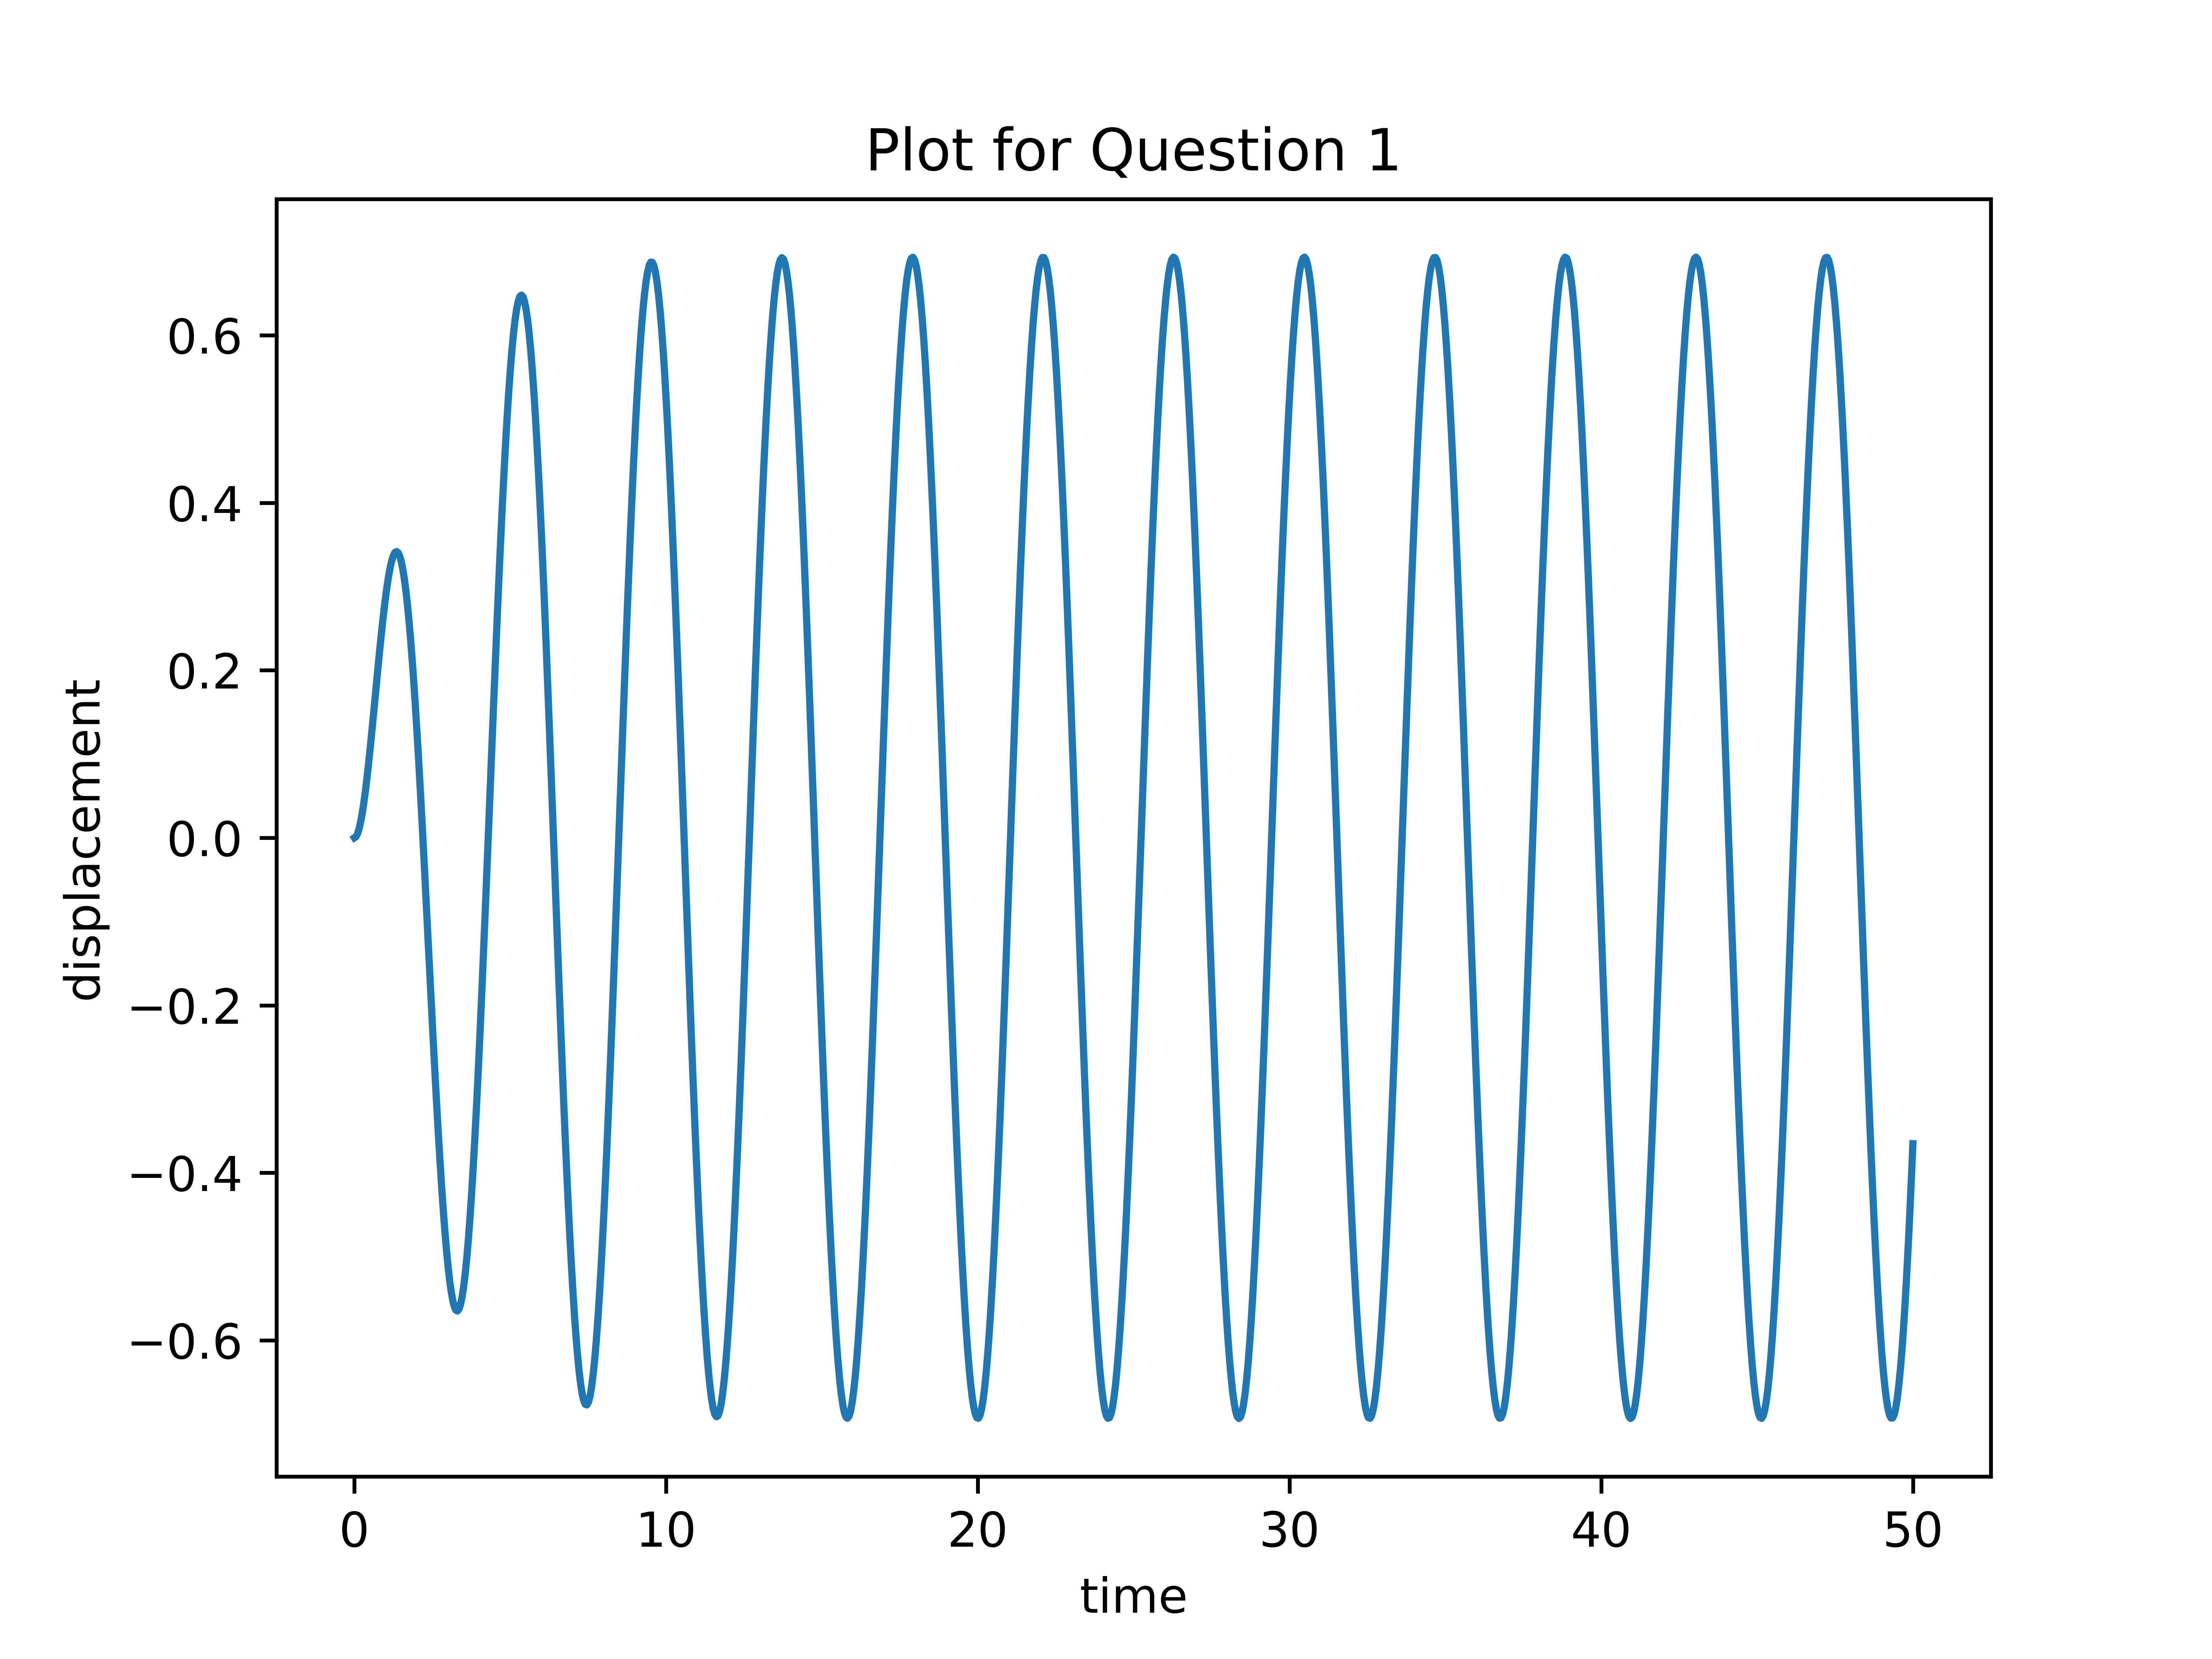
\includegraphics[scale=1]{images/fig1.png}
\end{center}

As we can see, it is a sinusoidal graph that initially starts with some damping but eventually it gets into a steady state of oscillations.
\pagebreak
\subsection{Question 2: Impulse Response with smaller decay}

The code for this is similar, we just need to change a few of the values that we send into our functions.

\begin{lstlisting}[language=Python]
def main():
    ...
    F2 = transfer(0.05,1.5)
    H2 = F2/X1
    ts2,xs2 = sp.impulse(H2,None,times)
    oneshotplot(2,ts2,xs2,'time','displacement',title="Plot for Question 2")
\end{lstlisting}

And we obtain the following graph:

\begin{center}
    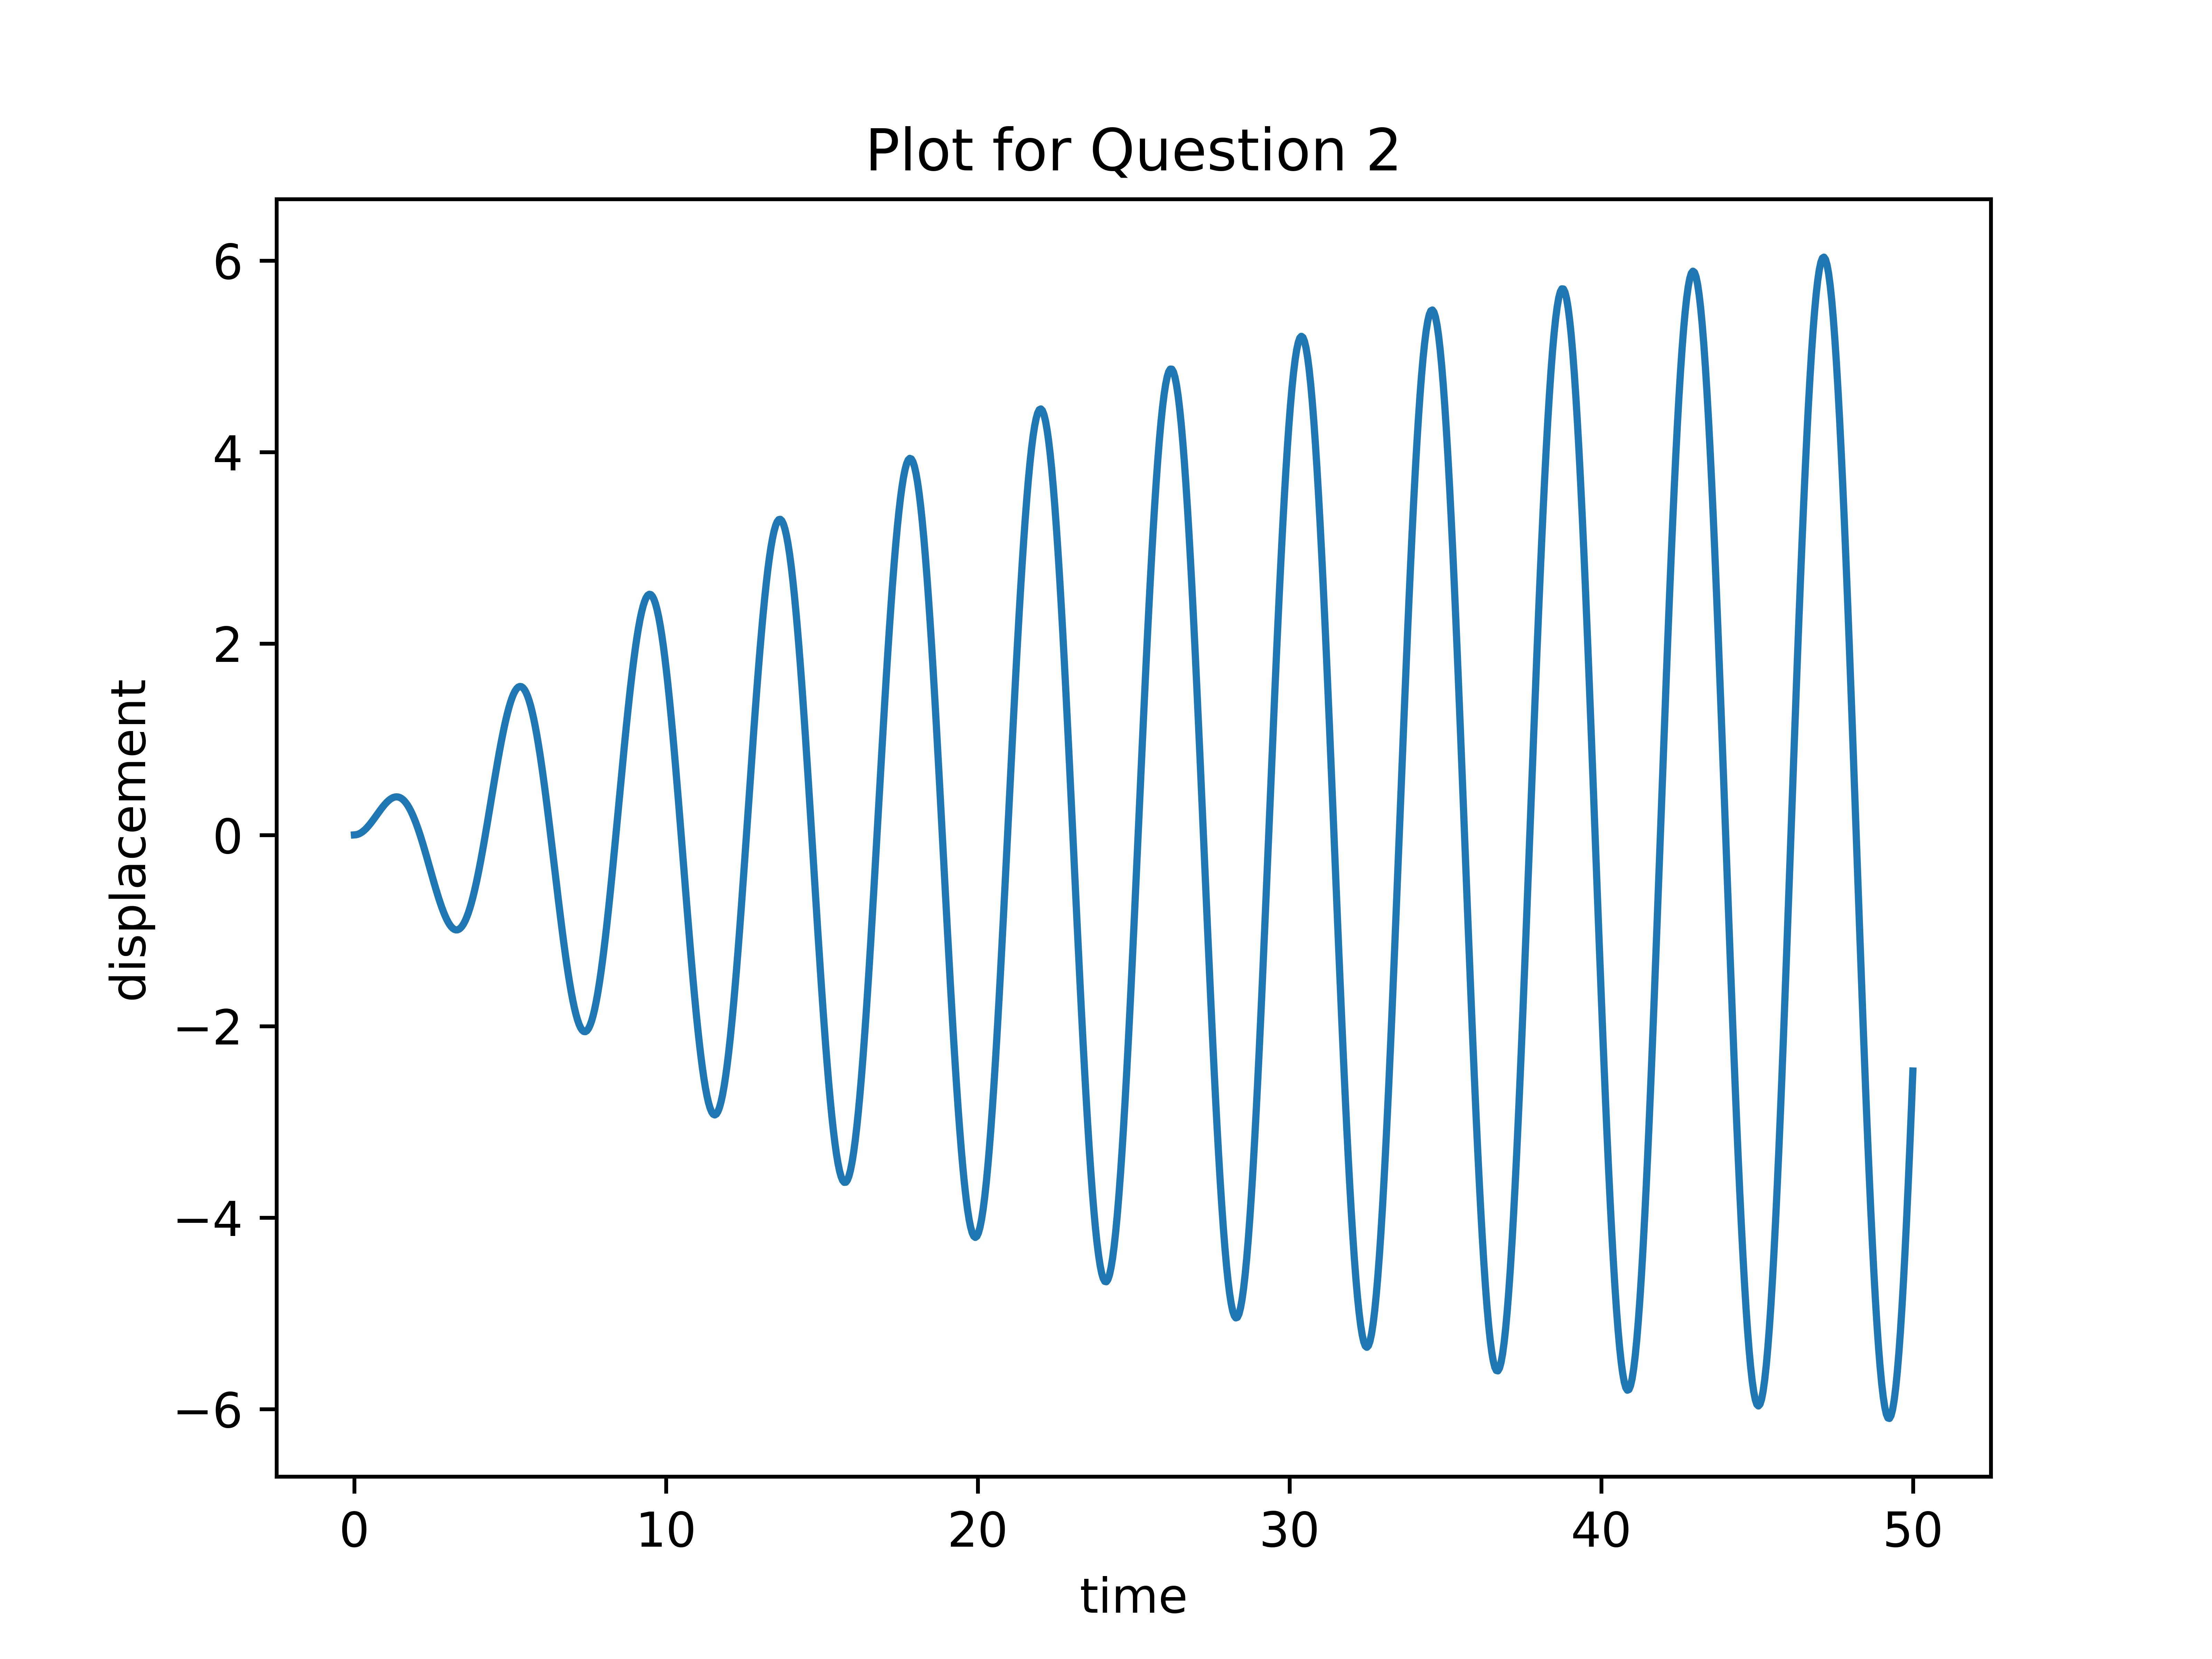
\includegraphics[scale=1]{images/fig2.png}
\end{center}

\pagebreak
\subsection{Question 3: Simulating the Impulse Response Calculation using \texttt{lsim}}
Here we loop over the different mentioned frequencies and plot each of them as a subplot.

\begin{lstlisting}[language=Python]
def main():
    ...
    myrange = np.arange(1.4,1.61,0.05)
    times1 = np.linspace(0,100,1000)
    plt.figure(3)
    for i,f in enumerate(myrange):
        currf = (np.cos(f*times1)*np.exp(-0.05*times1))*np.heaviside(times,0)
        _,y,_ = sp.lsim(H2,currf,times1)
        plt.subplot(3,2,i+1)
        plt.plot(times1,y,"-g")
    plt.suptitle("Impulse Response for different frequencies")
    plt.savefig("images/fig3.png",dpi=1000)
    plt.show()
\end{lstlisting}

And the plots obtained are as follows:
\begin{center}
    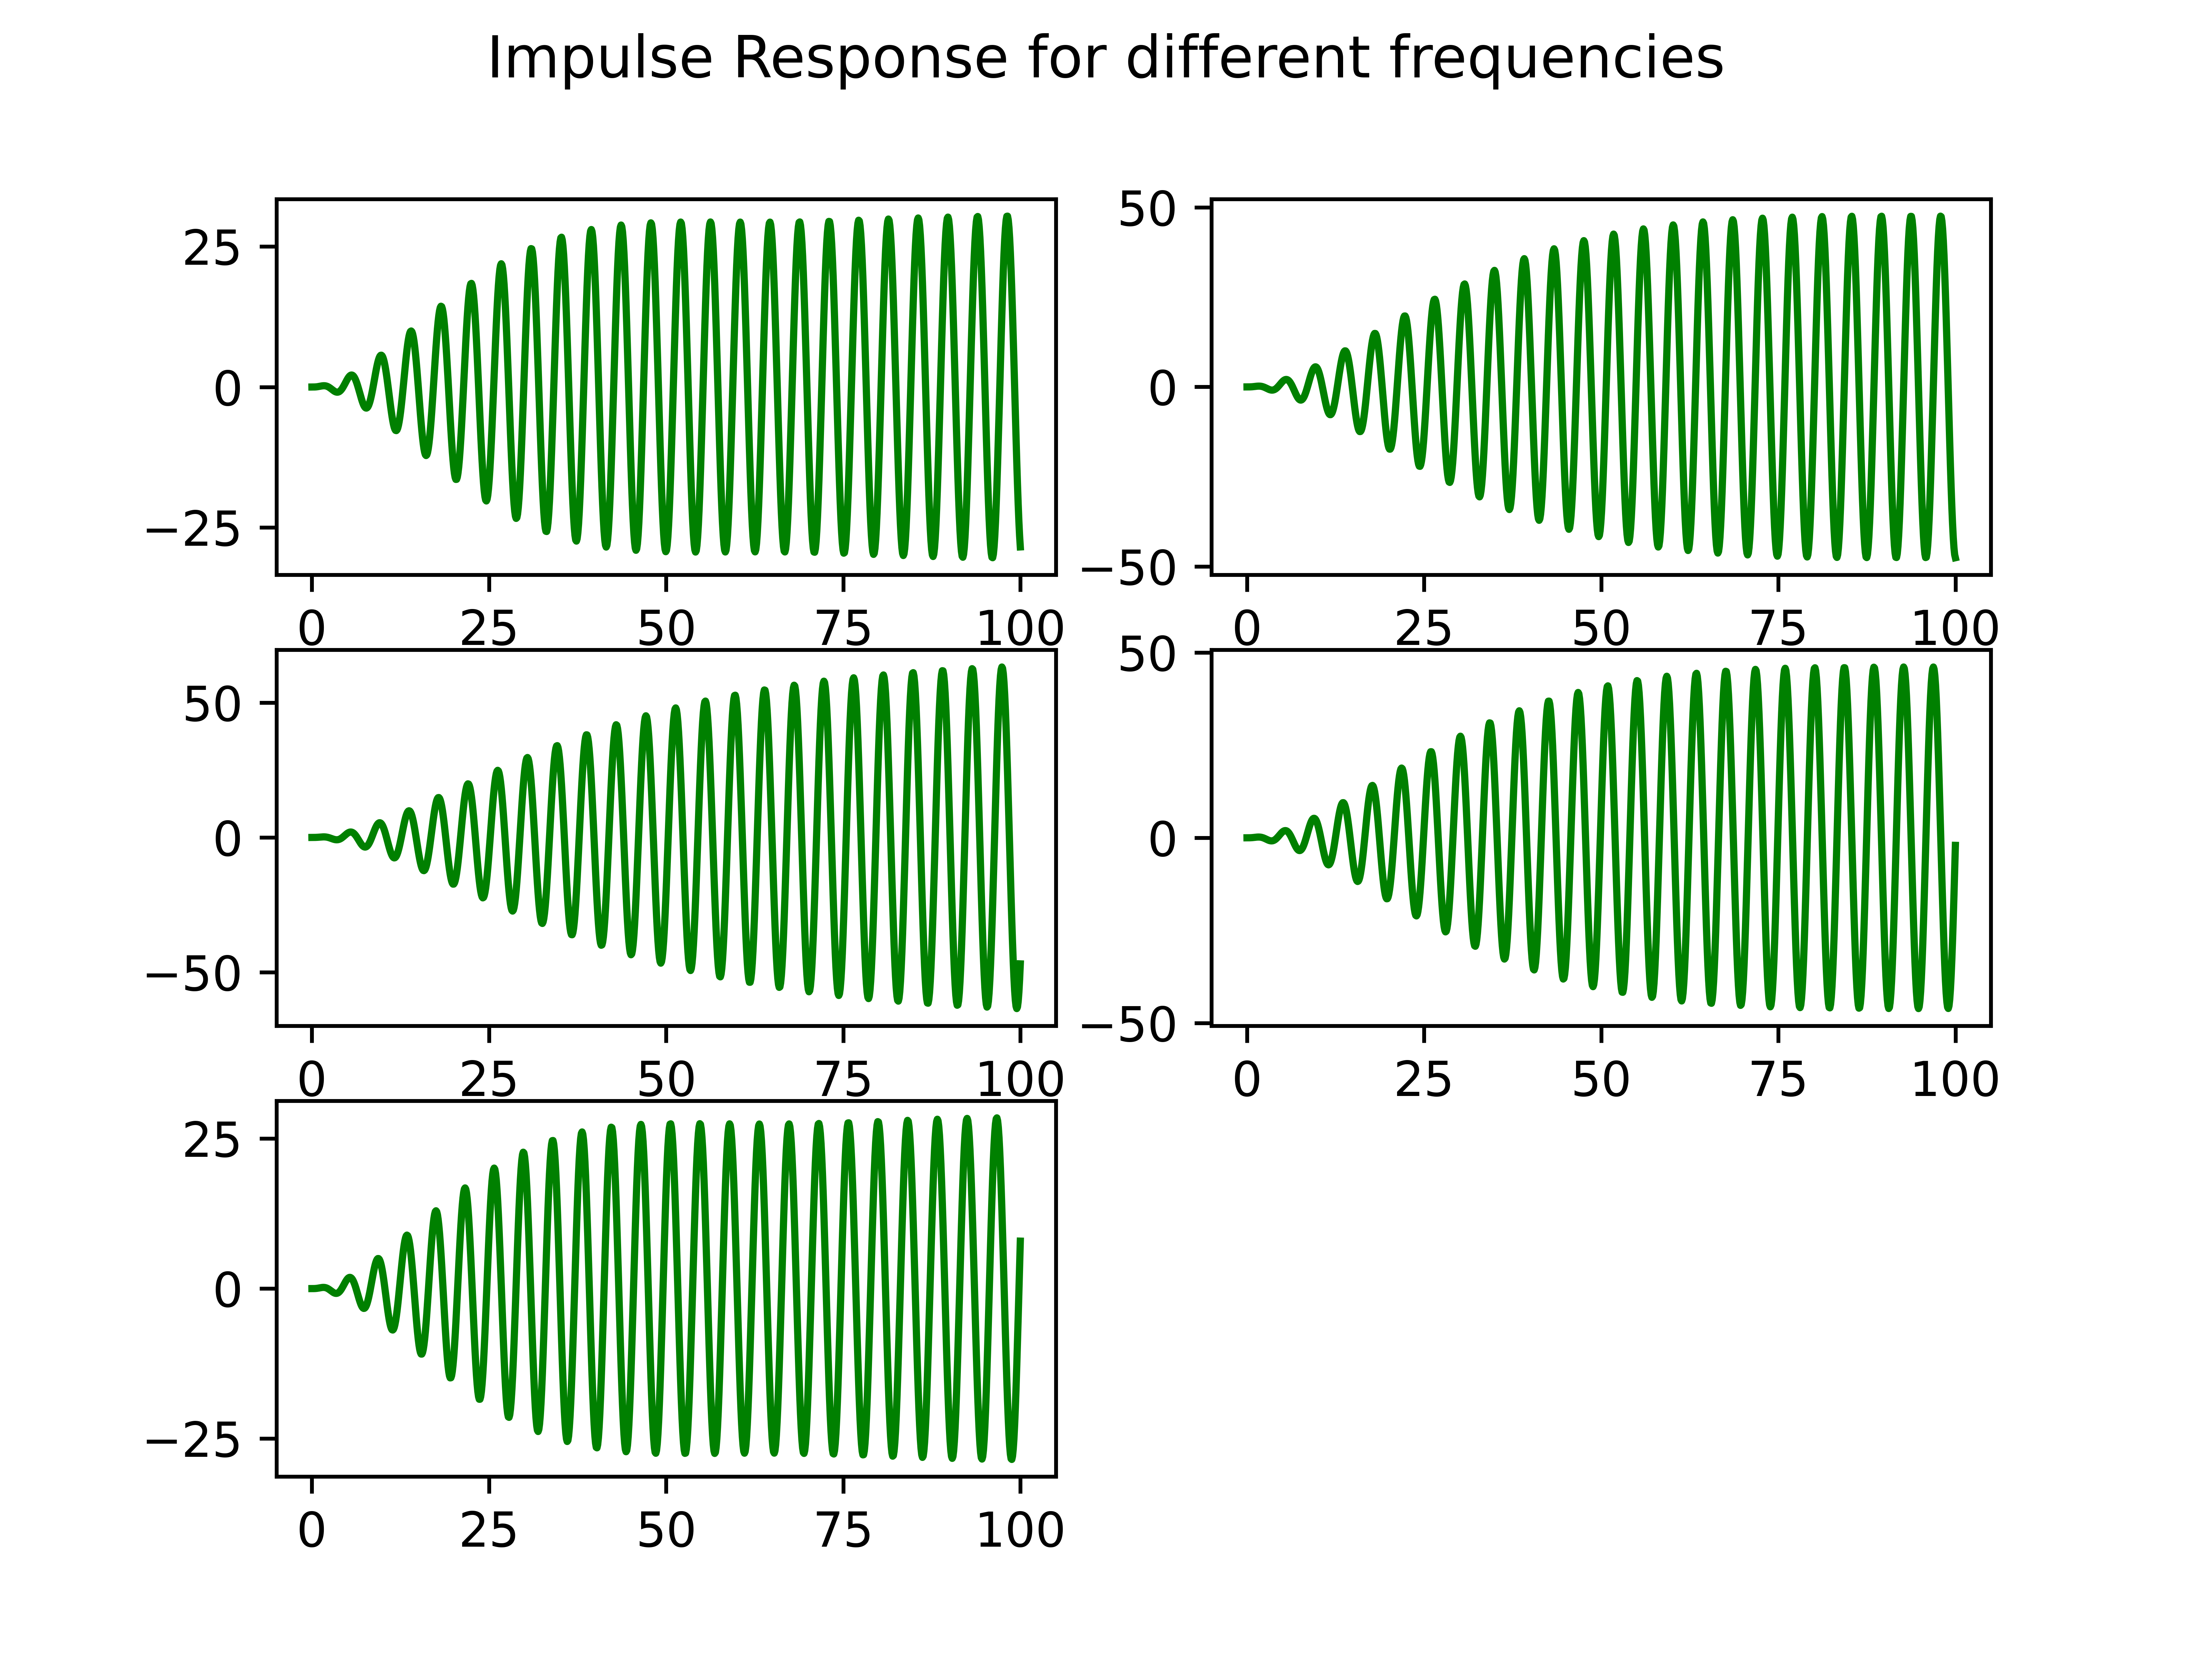
\includegraphics[scale=1]{images/fig3.png}
\end{center}
\pagebreak
\subsection{Question 4: Coupled Spring Problem}

First we need to convert the given differential equation into its corresponding Laplace Transform.

The given equations are $\ddot x + (x-y) = 0$ and $\ddot y + 2(y-x) = 0$, with initial conditions: $x(0)=1$, $\dot x(0) = y(0) = \dot y(0) = 0$

We take the Laplace Transform of these equations and we obtain:
$$s^2 X(s) - s + X(s) - Y(s) = 0 - (i)$$
$$s^2Y(s)+2Y(s)-2X(s)=0 - (ii)$$

On substituting $Y(s)$ from the first equation into the second, we obtain:

$$X(s) = \frac{s^2+2}{s^3+3s}$$ 
and $$Y(s) = \frac{2}{s^3+3s}$$

Hence, we now solve the two individually using the \texttt{impulse} function and plot them both on the same graph:

\begin{lstlisting}[language=Python]
def main():
    ...
    times2 = np.linspace(0,20,1000)
    Hx = LTIMore([1,0,2],[1,0,3,0])
    Hy = LTIMore([2],[1,0,3,0])
    tsx,xsx = sp.impulse(Hx,None,times2)
    tsy,xsy = sp.impulse(Hy,None,times2)
    plt.figure(4)
    plt.plot(tsx,xsx,label='x')
    plt.plot(tsy,xsy,label='y')
    plt.xlabel("Time")
    plt.ylabel("x, y")
    plt.legend()
    plt.title("Coupled Oscillations")
    plt.savefig("images/fig4.png",dpi=1000)
    plt.show()
\end{lstlisting}

And we obtain the following graph:
\begin{center}
    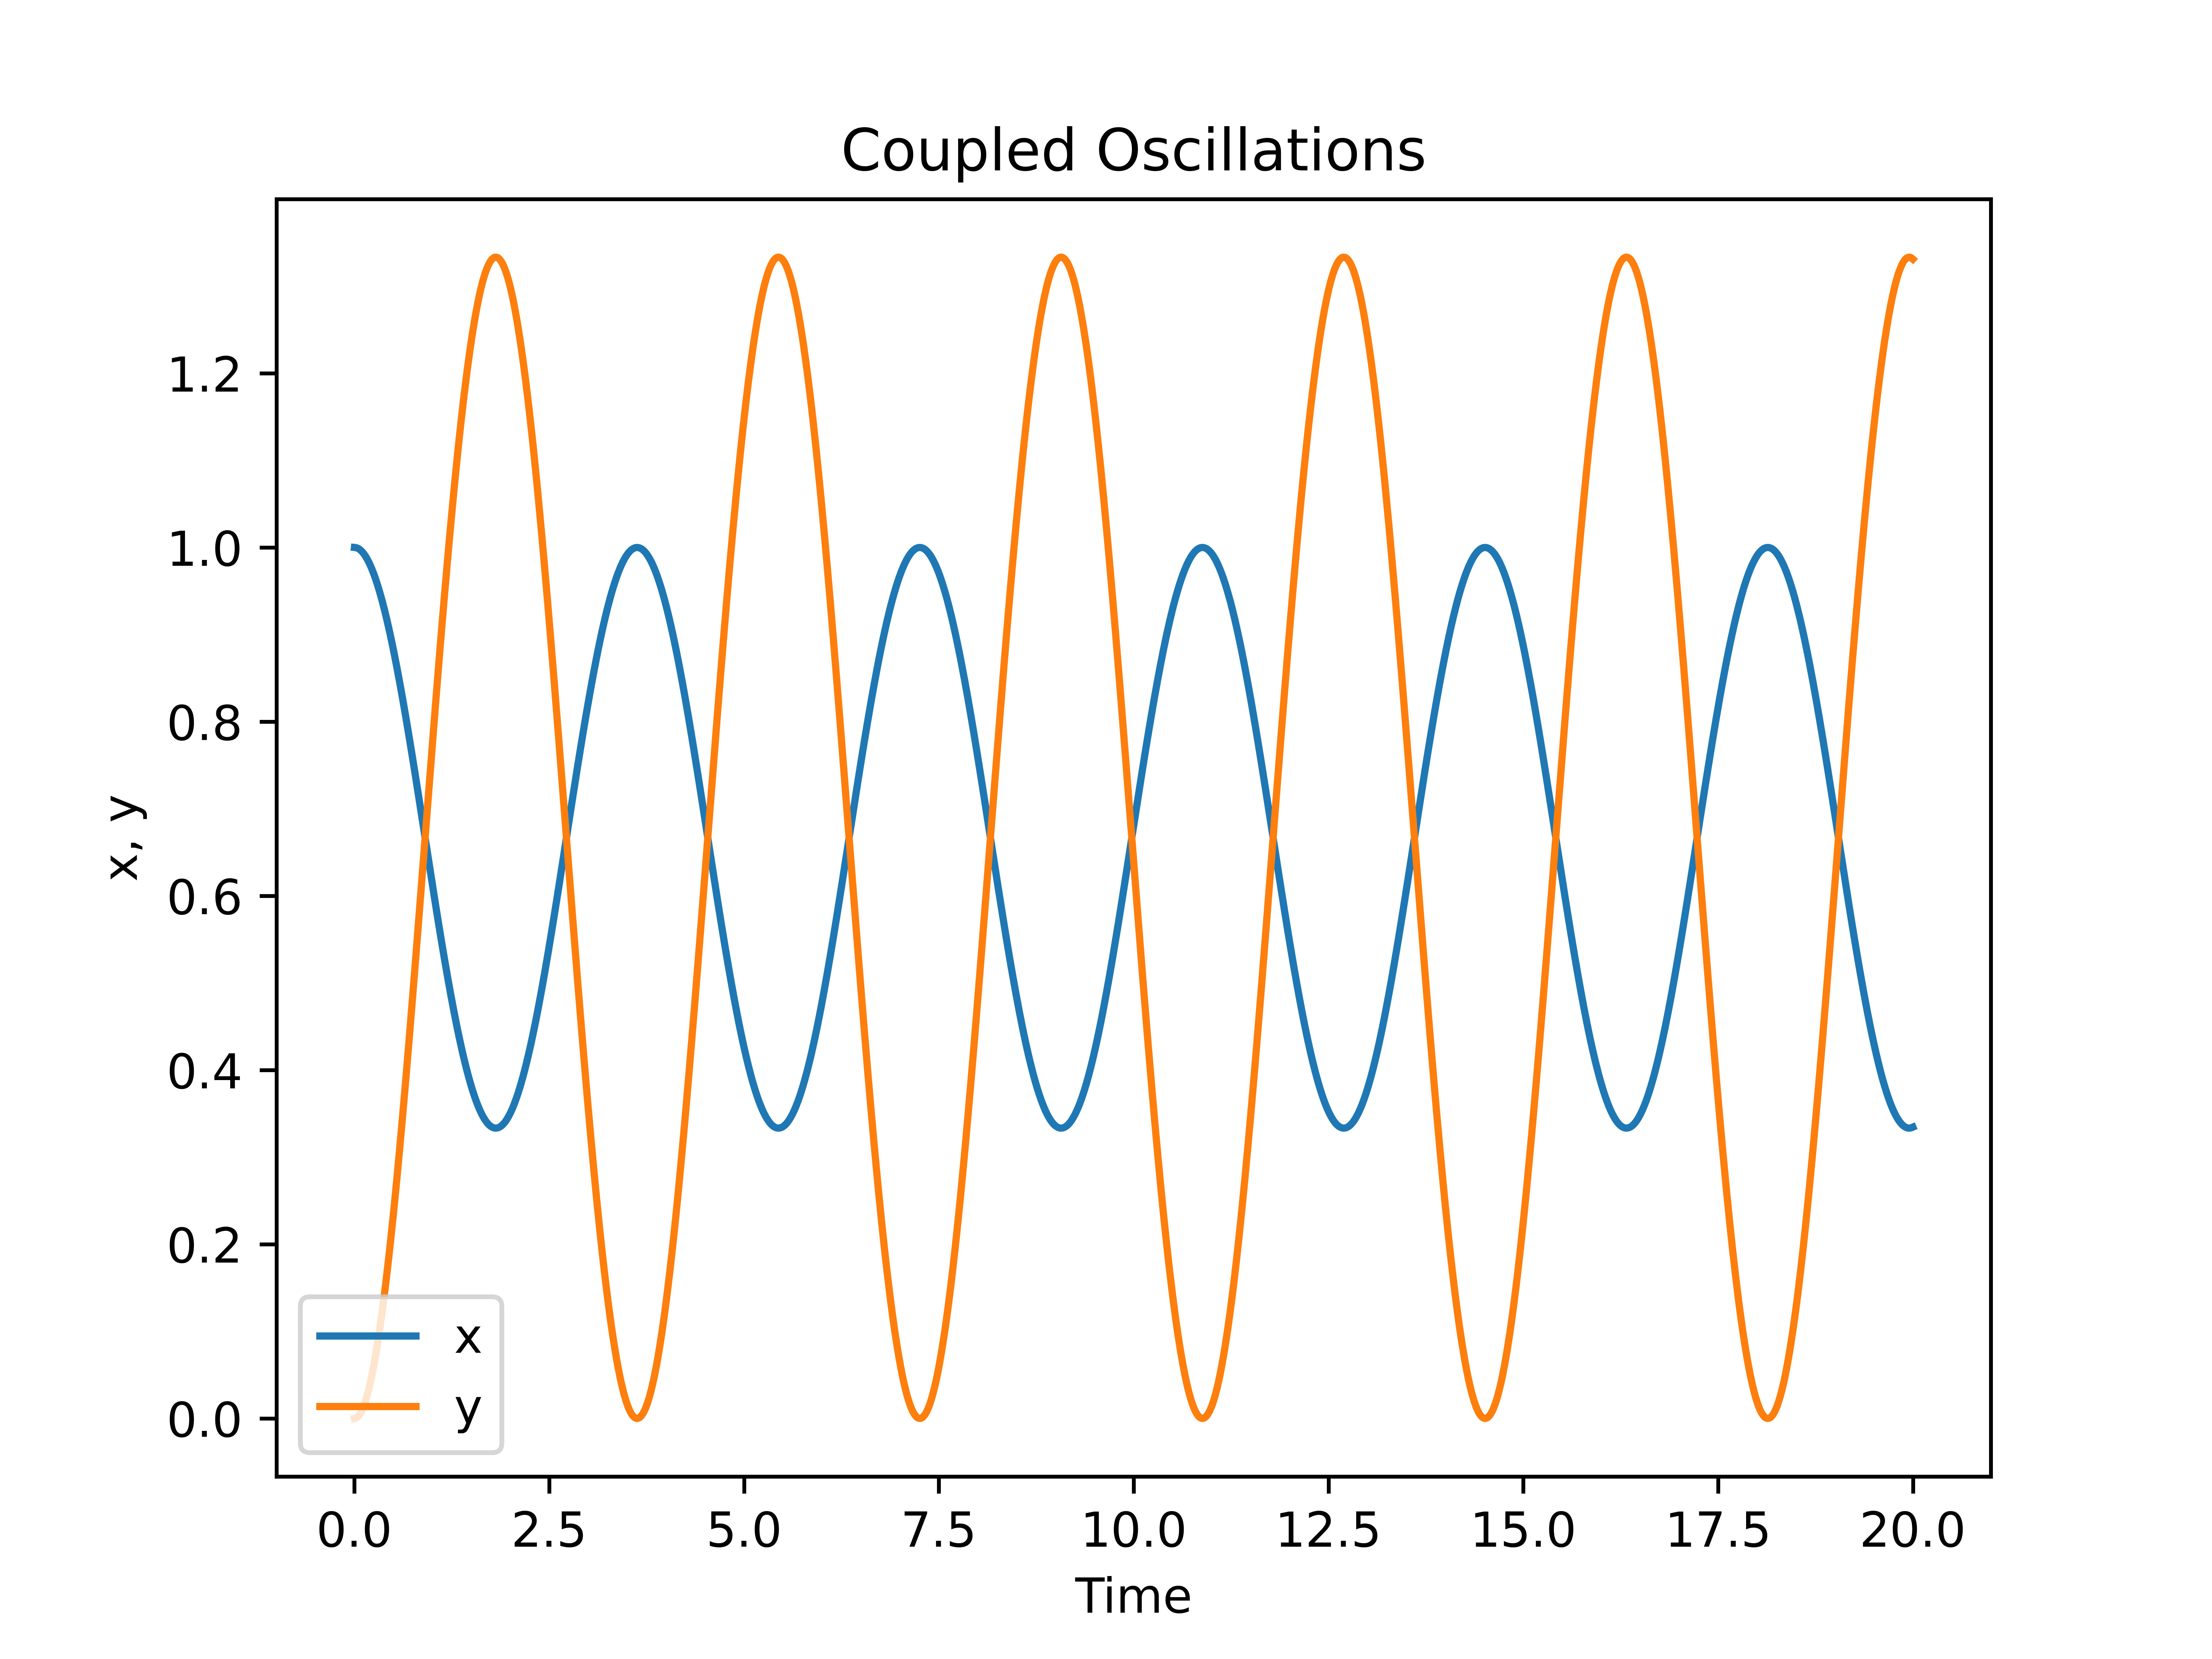
\includegraphics[scale=1]{images/fig4.png}
\end{center}

We see that the two curves are of the same frequency and seem to be exactly $180 \deg$ apart in phase and have different amplitudes.

\pagebreak
\subsection{Question 5: Bode Plots of 2 Port Network}
We are given the following 2 port network:

\begin{center}
    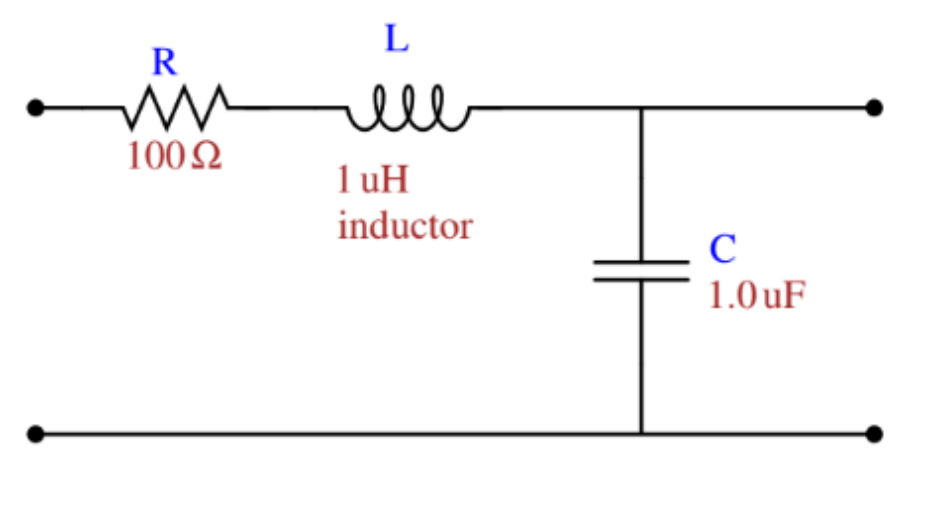
\includegraphics[scale=0.8]{RLC.png}
\end{center}

Once we solve the given 2 Port network, we obtain the following transfer function:

$$H(s) = \frac{10^6}{10^{-6} s^2 + 100 s + 10^6}$$

And then we obtain the Bode Plot of this.

\begin{lstlisting}[language=Python]
def main():
    ...
    H2p = LTIMore([1000000],[0.000001,100,1000000])
    w,mag,phase = sp.bode(H2p)
    plt.figure(5)
    plt.subplot(2,1,1)
    plt.semilogx(w,mag)
    plt.xlabel(r"$\omega$")
    plt.ylabel(r"$|H(s)|$")
    plt.subplot(2,1,2)
    plt.semilogx(w,phase)
    plt.xlabel(r"$\omega$")
    plt.ylabel(r"$\angle(H(s))$")
    plt.suptitle("Bode Plots for 2 Port Network")
    plt.savefig("images/fig5.png",dpi=1000)
    plt.show()
\end{lstlisting}

\begin{center}
    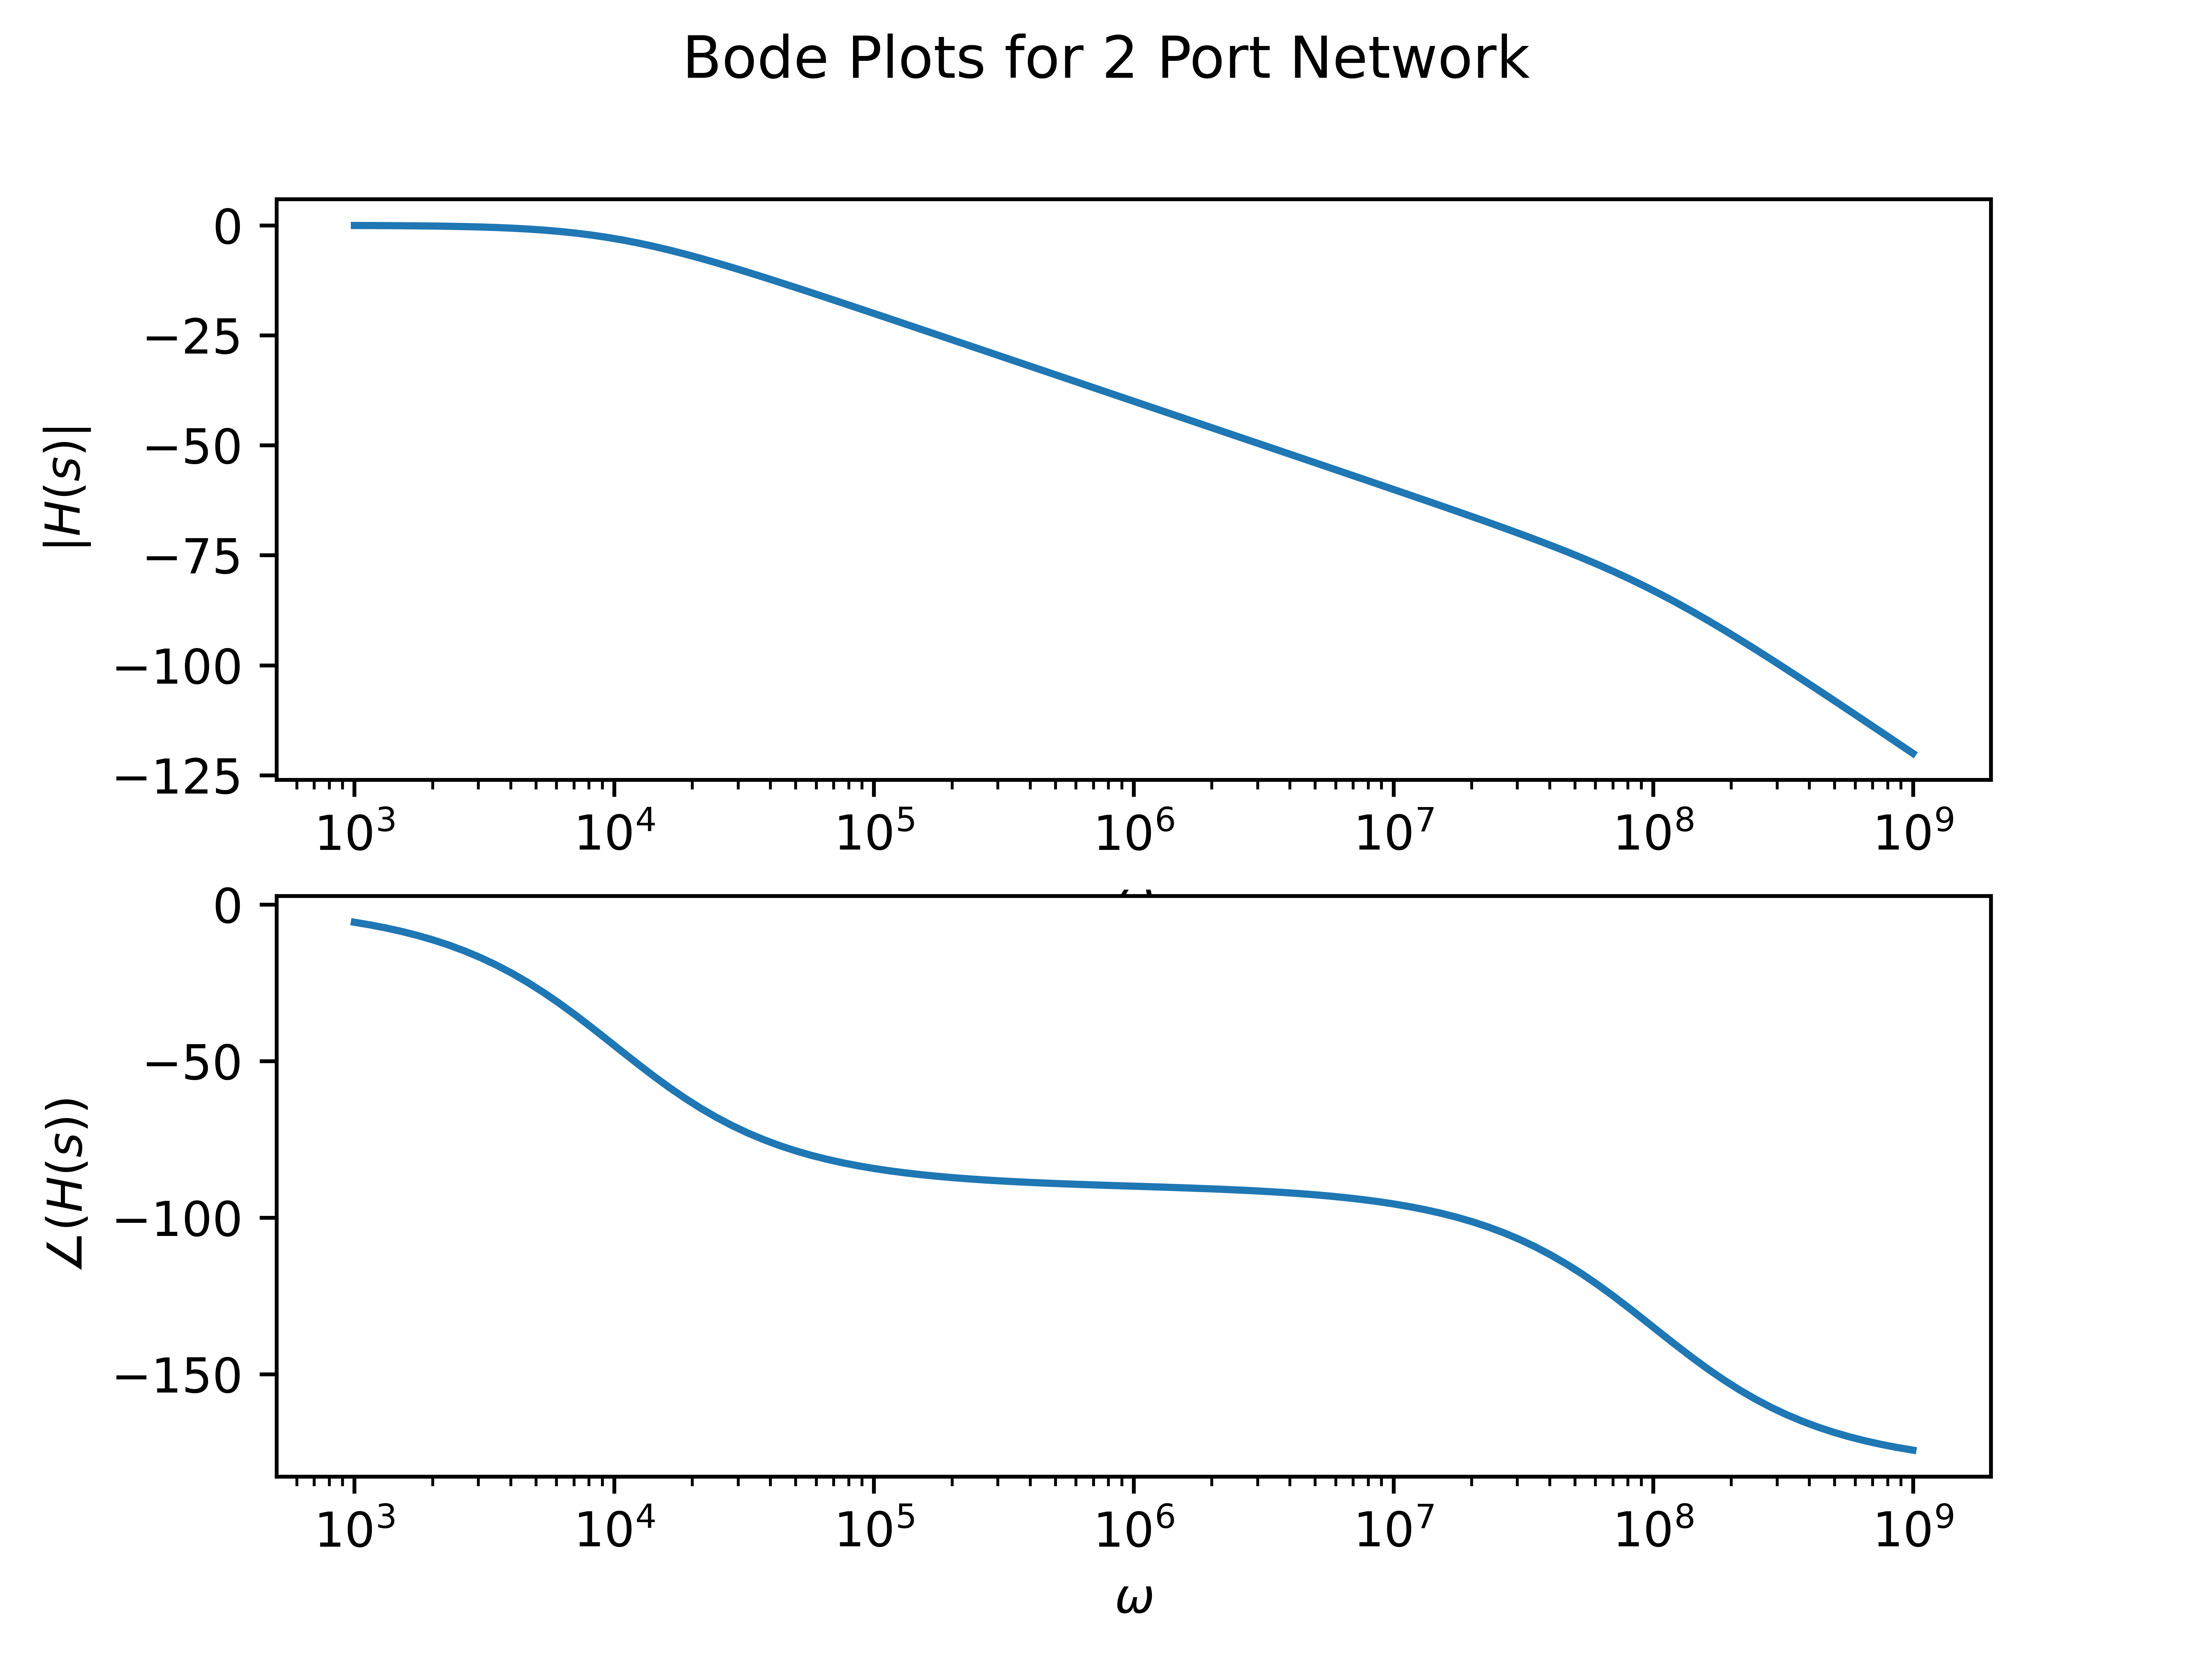
\includegraphics[scale=1]{images/fig5.png}
\end{center}
\pagebreak
\subsection{Question 6: Transient Response of 2 Port Network with given Inputs}
We are given the input function which we will use to simulate the response given the \texttt{lsim} function, and then see both the short term and long term responses.

We will simulate the function over 10 $\mu$s for the short term response and over 1ms for the long term response.

\begin{lstlisting}[language=Python]
def main():
    ...
    times3 = np.linspace(0,30*0.000001,1000)
    vi = np.multiply(np.cos(1000*times3)-np.cos(1000000*times3),np.heaviside(times3,0))
    _,y1,_ = sp.lsim(H2p,vi,times3)
    oneshotplot(6,times3,y1,'t',r'$v_{o}(t)$',r"Variation of $v_o(t)$ over 10$\mu$s")
    times4 = np.linspace(0,10*0.001,100000)
    vi = np.multiply(np.cos(1000*times4)-np.cos(1000000*times4),np.heaviside(times4,0))
    _,y2,_ = sp.lsim(H2p,vi,times4)
    oneshotplot(7,times4,y2,'t',r'$v_{o}(t)$',r"Variation of $v_o(t)$ over 1ms")
\end{lstlisting}

And we obtain the following graphs:
\begin{center}
    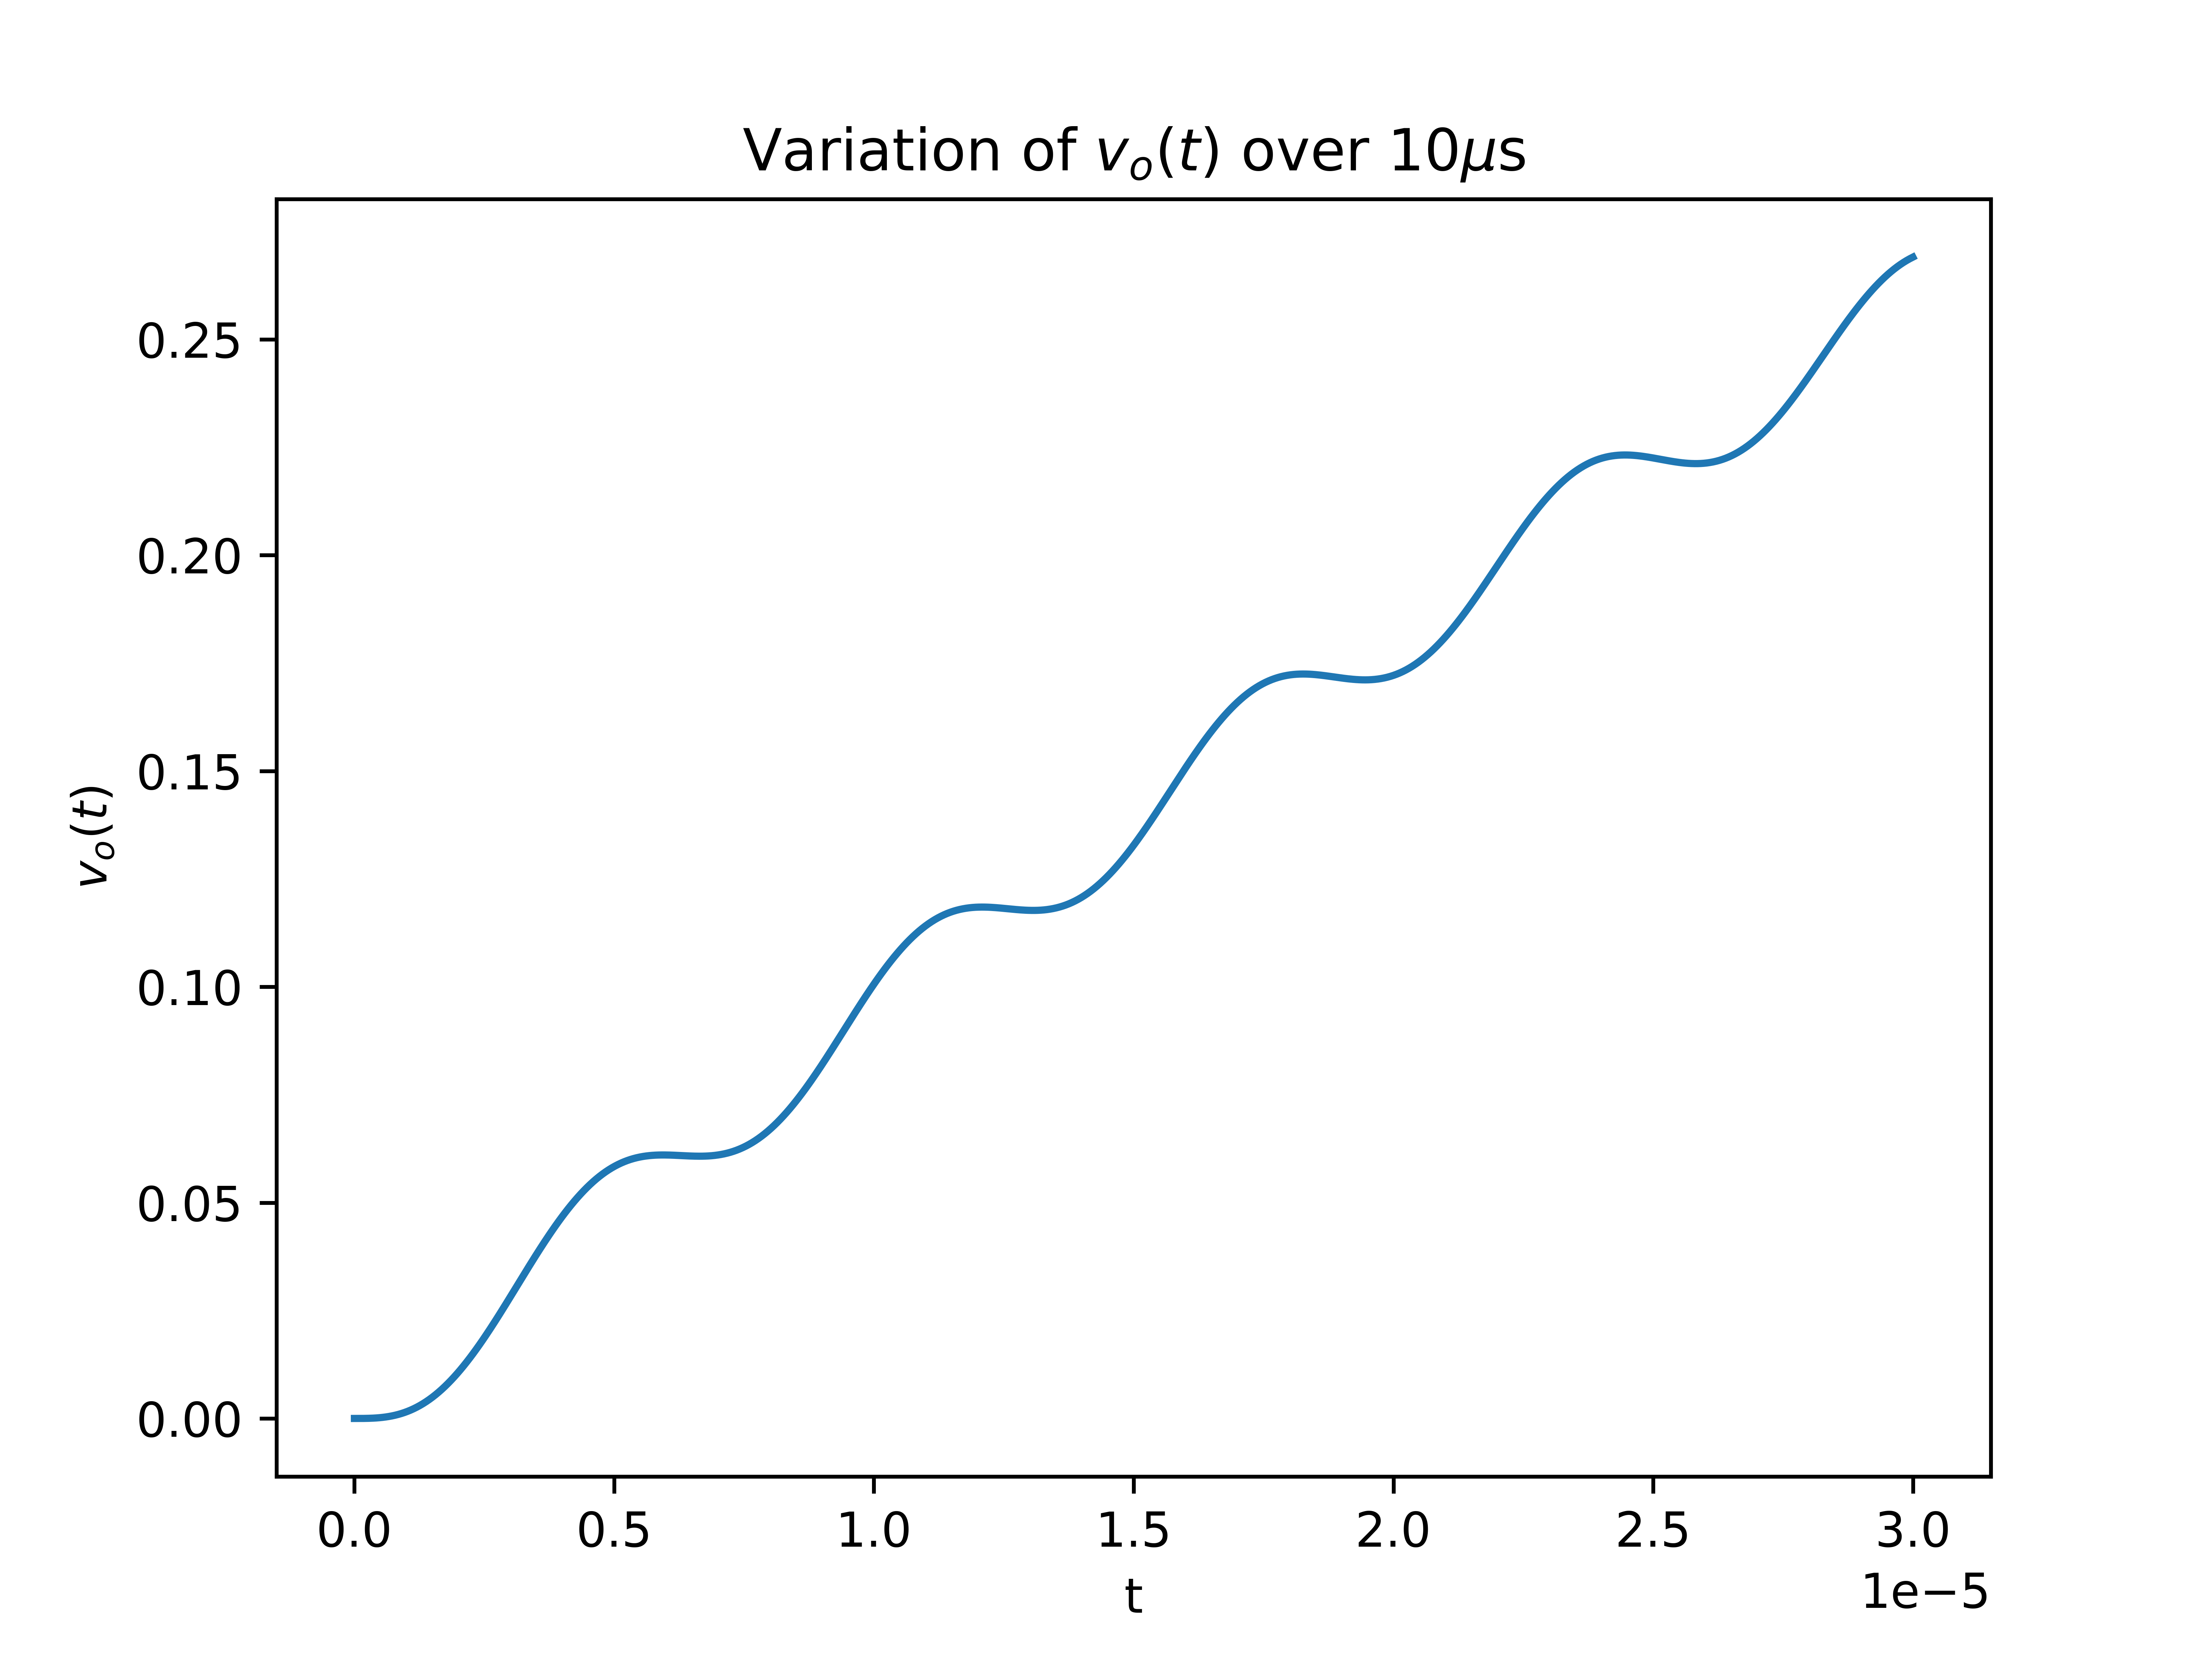
\includegraphics[scale=1]{images/fig6.png}
    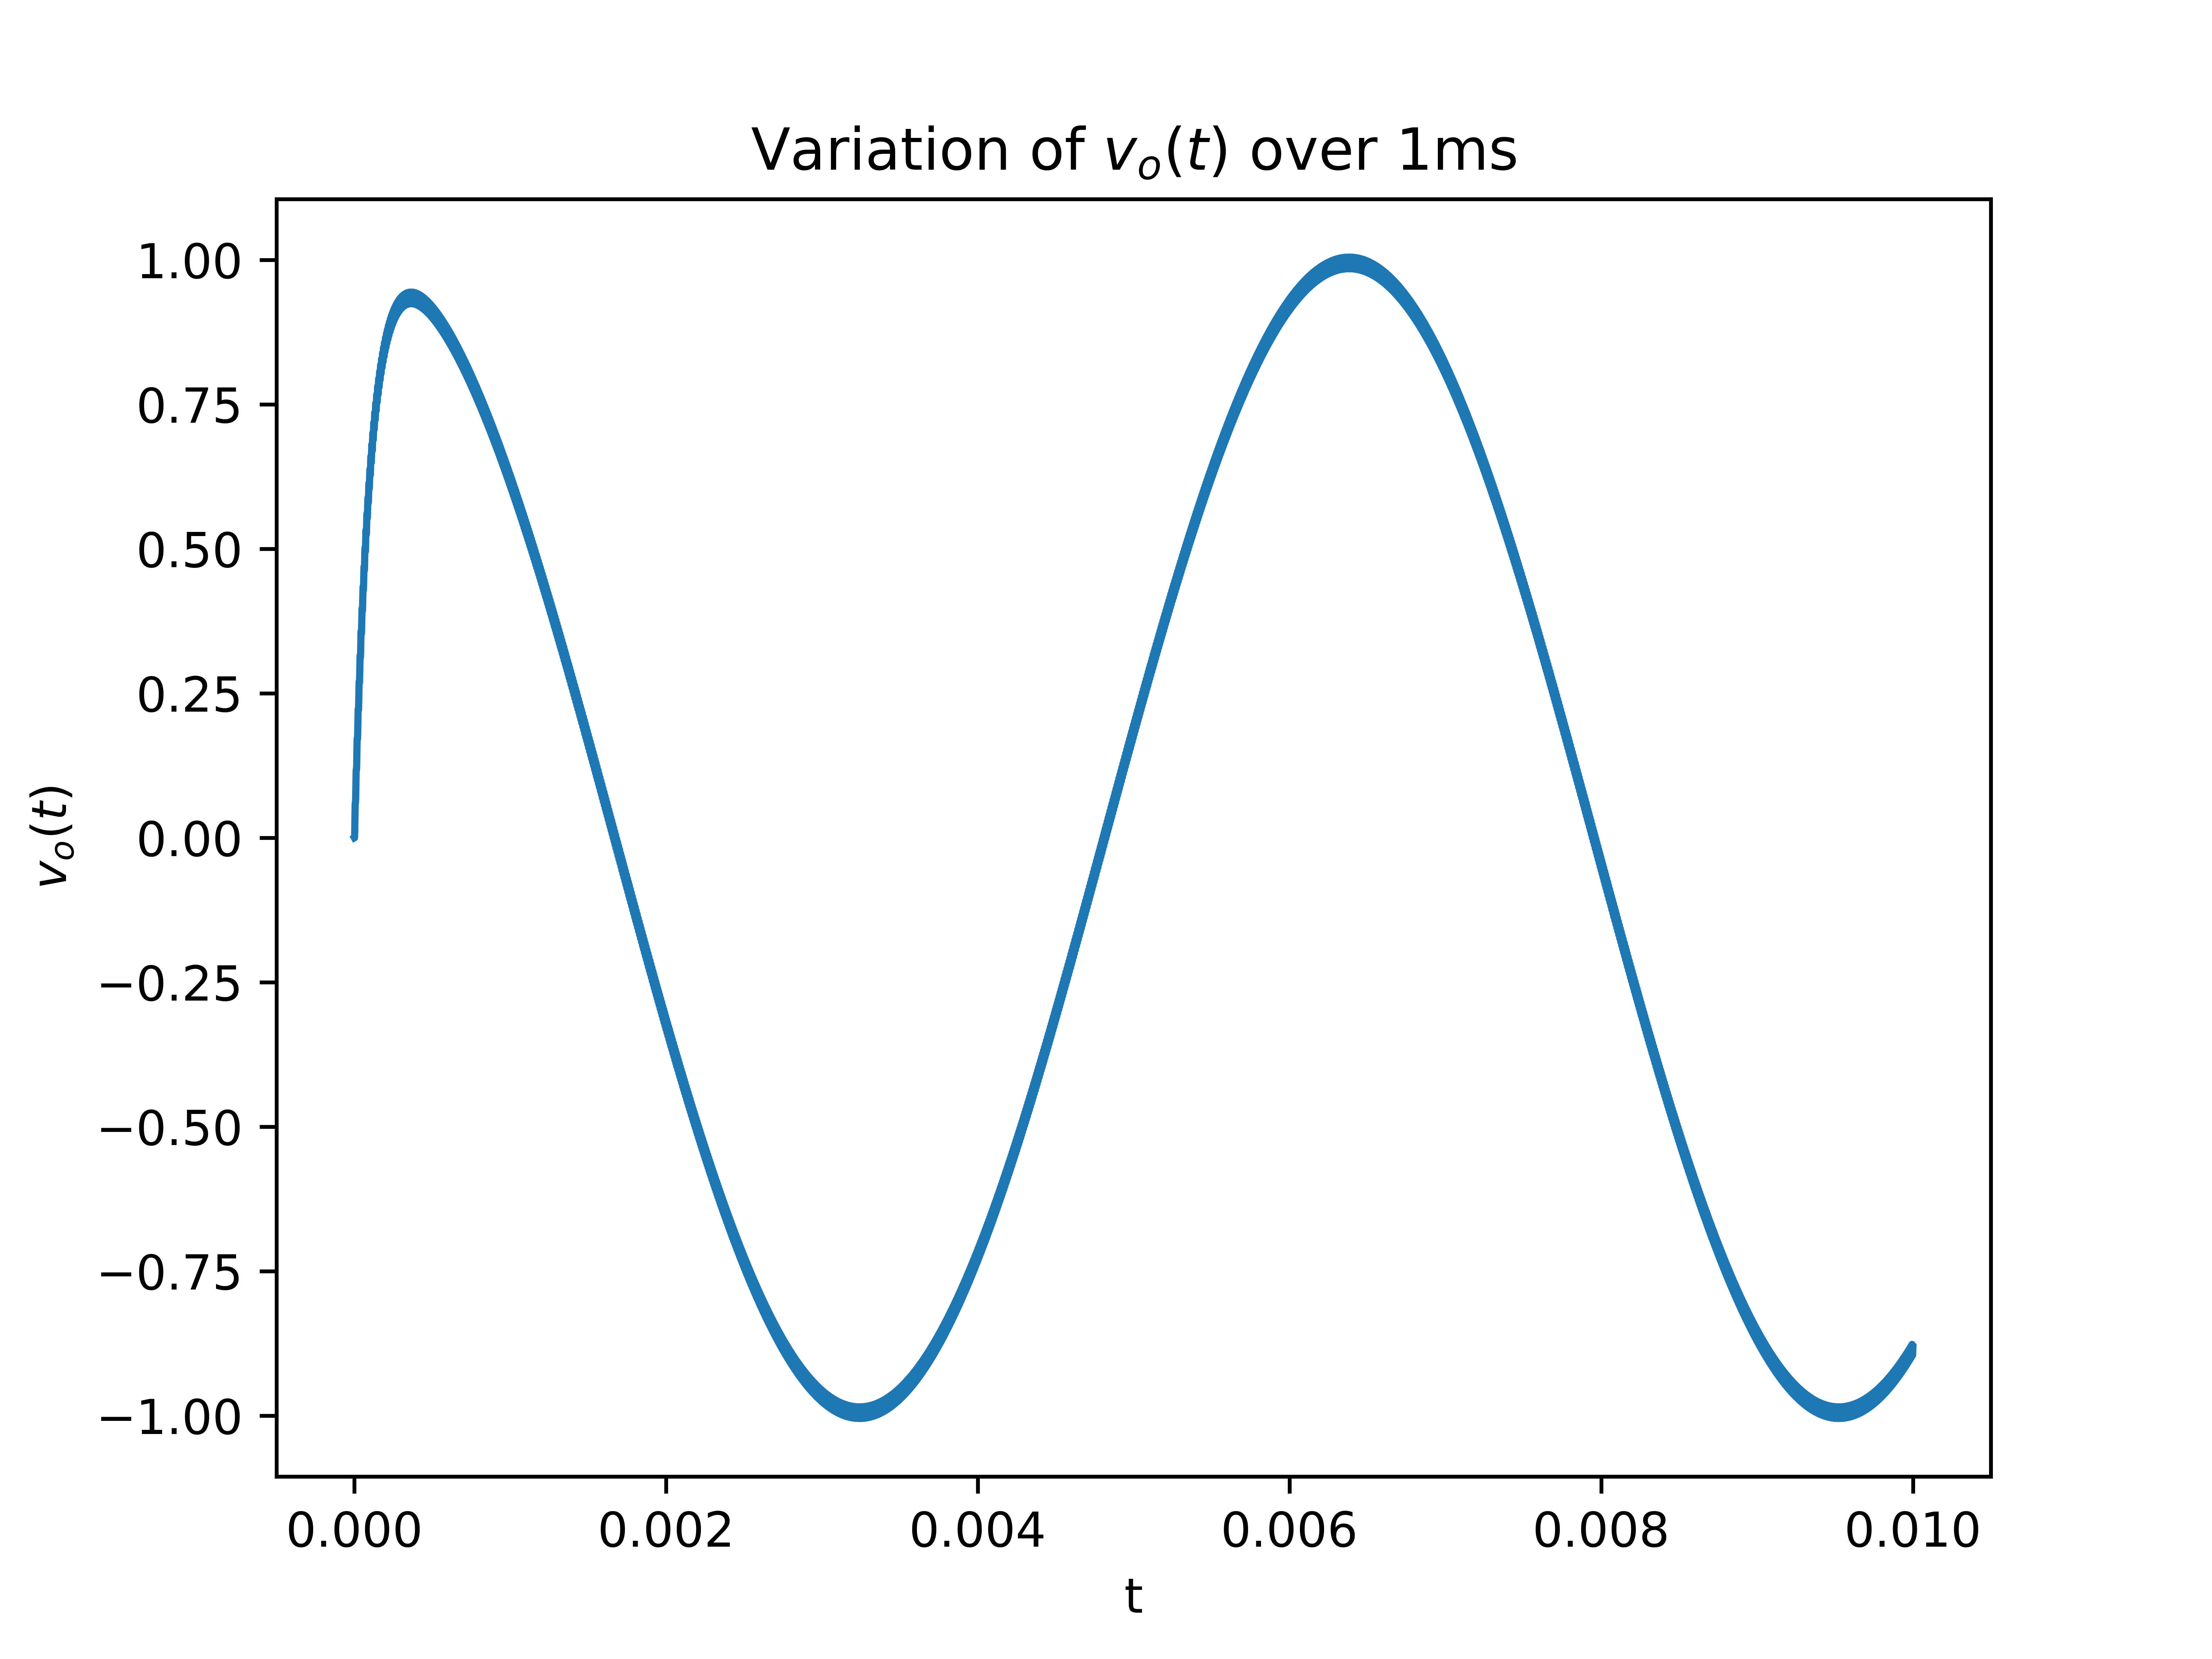
\includegraphics[scale=1]{images/fig7.png}
    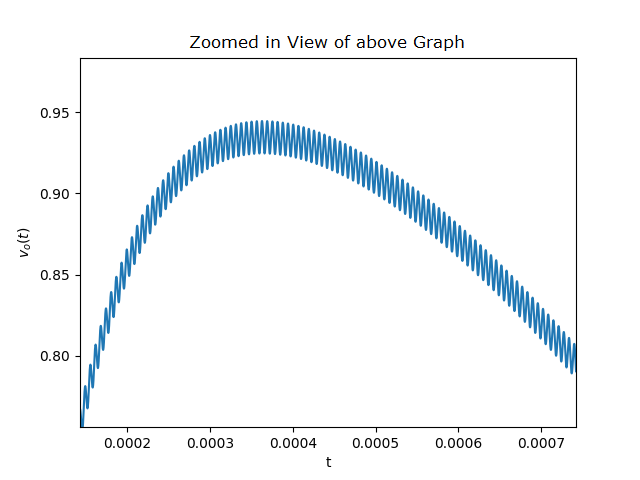
\includegraphics[scale=1.2]{images/fig8.png}
\end{center}

The Figure 7 is made of tiny oscillating values which are visible when we zoom in.
Their peak to peak values are about 0.02, and they are damped by the system. Effectively, the given RLC Circuit functions as a Low Pass filter and damps out the higher frequencies while keeping the low frequencies intact.

\section{Conclusions}
\begin{itemize}
    \item \texttt{scipy} provides a lot of useful signal processing functionality through the \texttt{signal} sub-module. 
    \item We used some of the available functions to analyze various systems, both mechanical and electrical
    \item We obtained Bode Plots and implemented a crude Low Pass filter with the given RLC Circuit that dampened the high frequencies.
\end{itemize}

\end{document}